\documentclass[class=report, crop=false, 12pt,a4paper]{standalone}
\usepackage{enumitem}
\usepackage{multicol}
\usepackage{graphicx}
\usepackage{float}
\usepackage{amsmath}
\usepackage{amssymb}
\usepackage{mathtools}
\usepackage{siunitx}
\usepackage{commath}
\usepackage{array}
\usepackage{natbib}
\usepackage{tikz}
\usepackage{cancel}
\usepackage[a4paper,width=150mm,top=25mm,bottom=25mm]{geometry}
\allowdisplaybreaks
\setlength{\parindent}{0pt}
\numberwithin{equation}{section}
\begin{document}
\begin{center}
  26/01/2021
\end{center}
The study of systems involving \textbf{moist air (dry air + water vapour)} is called psychrometrics.
\section{Air-Water Vapour Mixtures}
Moist air is found in:
\begin{itemize}[noitemsep]
  \item Nature;
  \item HVAC (heating, ventilation and air-conditioning) processes, where moisture (water vapour) is added or removed from the air;
  \item Steam turbines; and so on.
\end{itemize}
Moist air is a mixture of dry air and water vapour, where the \textbf{amount of dry air} is usually kept \textbf{constant} and the \textbf{amount of water vapour} may \textbf{change}. Two assumption are employed for air-water vapour properties :
\begin{enumerate}[noitemsep]
  \item \textbf{Dalton’s law} applies for the mixture, i.e. partial pressure $\longrightarrow p = p_a + p_v$
  \item Air and water vapour are each treated as \textbf{ideal gases, so is their mixture}.
\end{enumerate}
\section{Moist Air}
\begin{figure}[H]
  \centering
  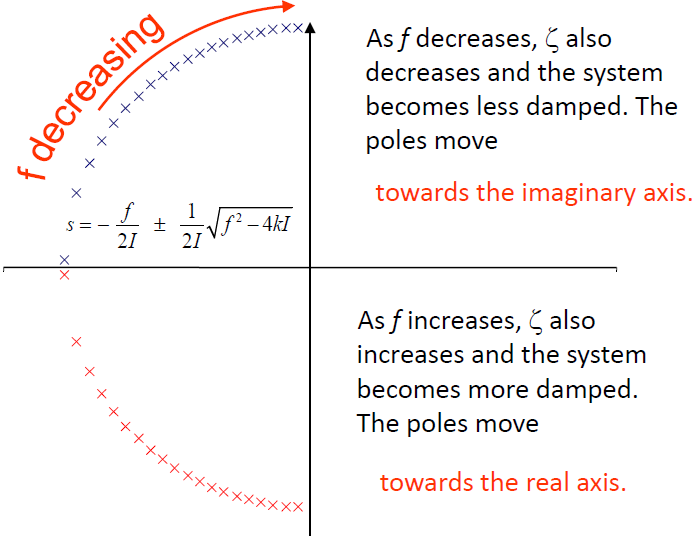
\includegraphics[width = 0.9 \textwidth]{../img/diagram98.png}
  \caption{}
\end{figure}
Equation of state of ideal gases:
\begin{gather}
  p = \frac{n R_u T}{V} = \frac{m(\frac{R_u}{M})T}{V} \\[5pt]
  p_a = \frac{n_a R_u T}{V} = \frac{m_a(\frac{R_u}{M_a})T}{V} \ \ \ \ \ p_a = y_ap\\[5pt]
  p_v = \frac{n_v R_u T}{V} = \frac{m_v(\frac{R_u}{M_v})T}{V} \ \ \ \ \ p_v = y_vp
\end{gather}
$p_v$ and $T$:
\begin{itemize}[noitemsep]
  \item Typical state: vapor is superheated;
  \item At $p_v = p_g$ (saturation pressure at $T$) $\longrightarrow$ Saturated Air (mixture of dry air and saturated water vapour); the mixture is said to be \textbf{saturated}.
\end{itemize}
\subsection{Moist Air Properties}
For a single component:
\begin{itemize}[noitemsep]
  \item \textbf{Two} independent, intrinsic properties are needed to define the state
\end{itemize}
For a two-component mixture (e.g. air-water vapor):
\begin{itemize}[noitemsep]
  \item \textbf{Three} independent, intrinsic properties are needed to define the state
  \begin{itemize}[noitemsep]
    \item Usually, two out of temperature, pressure
    and specific volume.
    \item Plus humidity ratio $\omega$ or relative humidity $\phi$ 
  \end{itemize}
\end{itemize}
\section{Specific Humidity}
The \textbf{specific humidity} or \textbf{humidity ratio} $\mathbf{\omega}$ is defined as:
\begin{gather}
  \omega = \frac{m_v}{m_a} = \frac{\text{mass of water vapour}}{\text{mass of dry air}}
\end{gather}
Using ideal gas law for both water vapour and dry air:
\begin{gather}
  \omega = \frac{R_u T}{M_a p_a V}\frac{M_v p_v V}{R_u T} = \frac{M_v p_v}{M_a p_a}
\end{gather}
Where, $T$ is temperature of the mixture measured by a convetional thermometer, called the dry bulb temperature denoted by $T_{db}$. \\\\
The molecular weights:
\begin{gather}
  M_v = 18 \ \ \ \ \ M_a = 28.96 \\[5pt]
  \frac{M_v}{M_a} \approx 0.622
\end{gather}
Dalton’s Law:
\begin{gather}
  p = p_a + p_v \\[5pt]
  \therefore p_a = p - p_v
\end{gather}
Specifiv Humidity:
\begin{gather}
  \omega = 0.622\frac{p_v}{p-p_v}
\end{gather}
\subsection{Moist Air Properties}
The humidity ratio is a parameter for determining other quantities: \\\\
Mass:
\begin{gather}
  m = m_m = m_a + m_v = m_a + \omega m_a \\[5pt]
  \therefore m = (1+\omega)m_a
\end{gather}
Energy:
\begin{gather}
  H = H_m = m_ah_a + m_vh_v \\[5pt]
  \therefore H = m_a(h_a + \omega h_v) \\[5pt]
  h = h_m = \frac{H}{m_a} = h_a + \omega h_v
\end{gather}
Humidity ratio is measured by a \textbf{hygrometer} in which a moist air sample is exposed to suitable chemicals until the moisture present is absorbed. The amount of water vapour is determined by weighing the chemicals.
\section{Relative Humidity}
\begin{gather}
  \phi = \frac{\text{partial pressure of water vapourat a temperature $T$ (in superheated state)}}{\text{saturation pressure of water vapour at the same temperature $T$ (or $T_{db}$)}} \\[5pt]
  \phi = \frac{p_v}{p_g}
\end{gather}
\begin{figure}[H]
  \centering
  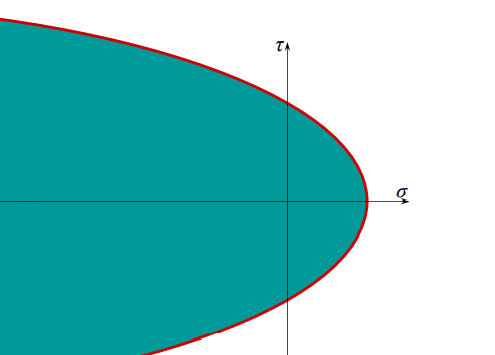
\includegraphics[width = 0.45 \textwidth]{../img/diagram99.png}
  \caption{}
\end{figure}
Consider ideal gas mixture:
\begin{gather}
  \phi = \frac{p_v}{p_g} = \frac{R_v T_v}{v_v}\frac{v_g}{R_v T_v} = \frac{v_g}{v_v} \\[5pt]
  \phi = \frac{v_g}{v_v} = \frac{p_v}{p_g} \leq 1.0 \ \ \ \text{always}
\end{gather}
\subsection{An Alternative Definition}
\begin{gather}
  \phi = \frac{\text{mole fraction of water vapour at a given $T$ and $P$ (in superheated state)}}{\text{mole fraction of water vapour at saturation at the same $T$ and $P$}} \\[5pt]
  \phi = \frac{y_v}{y_{v,sat}} = \frac{y_vp}{y_{v,sat}p} = \frac{p_v}{p_g}
\end{gather}
Relative humidity can be measured by \textbf{transducers} whose electrical characteristics change with relative humidity.
\subsection{Condensation of Moist Air}
Partial condensation of moist air can occur when temperature is reduced below a certain level:
\begin{figure}[H]
  \centering
  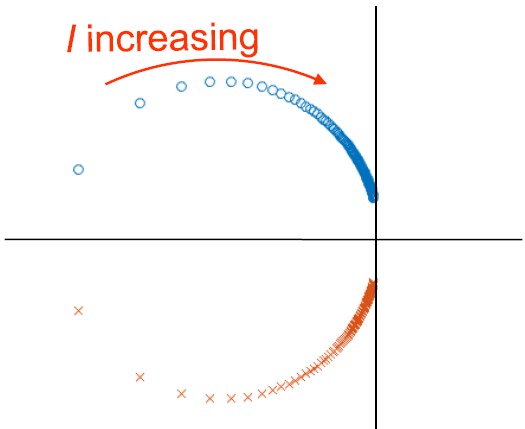
\includegraphics[width = 0.8 \textwidth]{../img/diagram100.png}
  \caption{Left: Condensate on windowpanes \ \ | \ \ Right: Dew on grass}
\end{figure}
The condensation process can be divided into the following stages:
\begin{itemize}[noitemsep]
  \item Superheated water vapour (state 1) is \textbf{cooled under constant system pressure} (thus the composition of moist air and partial pressure of vapour remain constant), until it reaches \textbf{the dew point} (state d);
  \begin{itemize}[noitemsep]
    \item The saturation temperature corresponding to pv is called the dew point temperature $(T_{dp})$.
  \end{itemize}
  \item Vapour starts to \textbf{condense when the moist air is cooled below} $\mathbf{T_dp}$.
  \item Further cooling leads to more condensate until the dry air, saturated vapour and liquid water \textbf{reach equilibrium}.
  \item At the final state, the system consists of \textbf{saturated air} (state 2) and \textbf{saturated liquid} (state 3) at the final temperature. The saturated vapour (state 2) has a partial pressure of the saturation pressure $p_{g2}$
\end{itemize}
\begin{figure}[H]
  \centering
  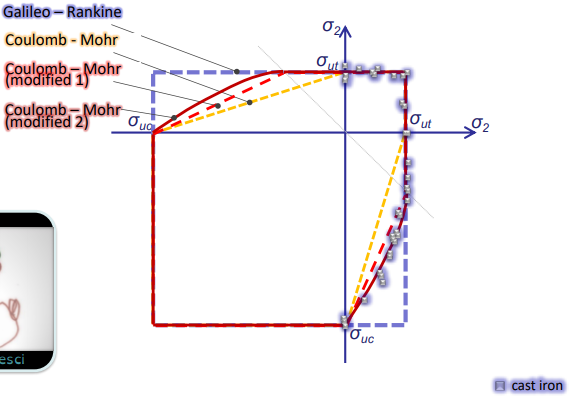
\includegraphics[width = 1 \textwidth]{../img/diagram101.png}
  \caption{}
\end{figure}
\section{Adiabatic Saturation Temperature $T_{as}$}
\begin{figure}[H]
  \centering
  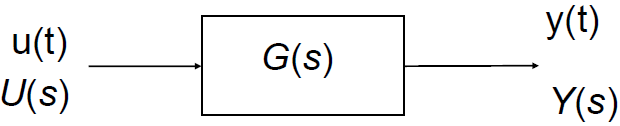
\includegraphics[width = 1 \textwidth]{../img/diagram102.png}
  \caption{}
\end{figure}
The idea of the above \textbf{Adiabatic Saturator} is to determine the unknown humidity ratio at the inlet based on values of $p$, $T$ and \textbf{Adiabatic Saturation Temperature} $\mathbf{T_{as}}$.
\subsection{The Adiabatic Saturation Analysis}
Assumptions:
\begin{itemize}[noitemsep]
  \item Steady state
  \item $\Delta$KE = $\Delta$PE = 0
  \item Adiabatic process
  \item Constant pressure process
  \item Air and water vapor are ideal gases
\end{itemize}
Mass Balances:
\begin{align}
  \text{Dry air balance:} \ \ \ &\dot{m}_{a,1} = \dot{m}_{a,2} = \dot{m}_a \\[5pt]
  \text{Water balance:} \ \ \ &\dot{m}_{v,1} + \dot{m}_L = \dot{m}_{v,2} \\[5pt]
  \longrightarrow \ \ \ &\omega\dot{m}_a + \dot{m}_L = \omega'\dot{m}_a \\[5pt]
  \longrightarrow \ \ \ &\dot{m}_L = \dot{m}_a(\omega'-\omega) = \dot{m}_a(\omega_2-\omega_1)
\end{align}
1st Law for Open System, energy balance:
\begin{gather}
  \frac{\dif E_{CV}}{\dif t} = \dot{Q} + \dot{W} + \sum_{in}\dot{m}_{in}\left(h+\frac{v^2}{2}+gz\right)_{in} - \sum_{out}\dot{m}_{out}\left(h+\frac{v^2}{2}+gz\right)_{out} \\[5pt]
  \cancel{\frac{\dif E_{CV}}{\dif t}} = \cancel{\dot{Q}} + \cancel{\dot{W}} + \sum_{in}\dot{m}_{in}\left(h+\cancel{\frac{v^2}{2}}+\cancel{gz}\right)_{in} - \sum_{out}\dot{m}_{out}\left(h+\cancel{\frac{v^2}{2}}+\cancel{gz}\right)_{out} \\[5pt]
  0 = \dot{m}_{a}h_{a,1} + \dot{m}_{v,1}h_{v,1} + \dot{m}_{L}h_{L} - \dot{m}_{a}h_{a,2} - \dot{m}_{v,2}h_{v,2} \\[5pt]
  0 = \dot{m}_{a}h_{a,1} + \omega_{1}\dot{m}_{a}h_{v,1} + \dot{m}_{a}(\omega_2 - \omega_1)h_{L} - \dot{m}_{a}h_{a,2} - \omega_2\dot{m}_{a}h_{v,2} \\[5pt]
  0 = h_{a,1} + \omega h_{v,1} + (\omega'-\omega)h_{f,2} - h_{a,2} - \omega'h_{v,2} \\[5pt]
  \longrightarrow \omega h_{v,1} - \omega h_{f,2} = (h_{a,2} - h_{a,1}) + \omega'(h_{v,2} - h_{f,2}) \\[5pt]
  \longrightarrow \omega = \frac{(h_{a,2} - h_{a,1}) + \omega'(h_{v,2} - h_{f,2})}{h_{v,1} - h_{f,2}} \\[5pt]
  h_v \approx h_g(T) \\[5pt]
  \omega = \frac{[h_a(T_{as}) - h_a(T)] + \omega'[h_g(T_{as}) - h_f(T_{as})]}{h_g(T) - h_f(T_{as})} \\[5pt]
  \omega' = 0.622\frac{p_g(T_{as})}{p - p_g(T_{as})}
\end{gather}
\section{Wet-bulb Temperature $T_{wb}$}
\subsubsection{Dry-bulb Temperature $T_{db}$}
\begin{itemize}[noitemsep]
  \item Measured by a normal thermometer placed in the mixture.
\end{itemize}
\subsubsection{Wet-bulb Temperature $T_{wb}$}
\begin{itemize}[noitemsep]
  \item Measured by a wet-bulb thermometer, which is an ordinary liquid-in-glass thermometer whose bulb is enclosed by a wick moistened with water.
  \item $T_{wb}$ is a close approximation of the adiabatic saturation temperature.
  \item $T_{wb}$ is used in place of $T_{as}$ to determine $\omega$ in the adiabatic saturator.
\end{itemize}
\begin{gather}
  \omega = \frac{[h_a(T_{wb}) - h_a(T_{db})] + \omega'[h_g(T_{wb}) - h_f(T_{wb})]}{h_g(T_{db}) - h_f(T_{wb})}
\end{gather}
\begin{figure}[H]
  \centering
  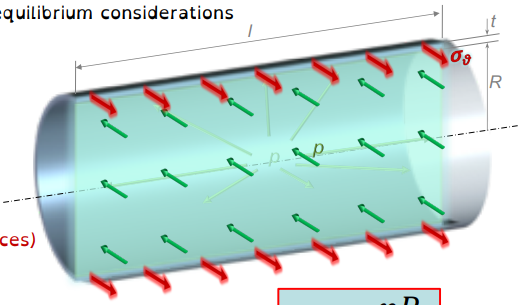
\includegraphics[width = 0.95 \textwidth]{../img/diagram103.png}
  \caption{}
\end{figure}
\section{Psychrometers}
\begin{figure}[H]
  \centering
  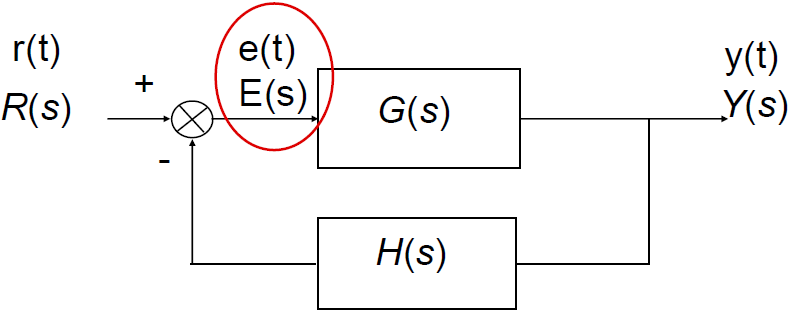
\includegraphics[width = 0.9 \textwidth]{../img/diagram104.png}
  \caption{(a) Sling Psychrometers \ \ | \ \ (b) Aspirating Psychrometers}
\end{figure}
These are the devices to measure temperature and provide the humidity ratio.
\end{document}